\documentclass[journal]{IEEEtran}
\usepackage{graphicx}
\usepackage{amsmath}
\usepackage{booktabs}
\usepackage{url}
\usepackage[hidelinks]{hyperref}
\graphicspath{{figures/}}

\begin{document}

\title{Launch-Blind Product Viability Estimation from Specifications via LLM Aspect Bridging}

\author{Raj~Jagtap%
\thanks{R. Jagtap is an undergraduate student of Computer Science and Engineering. This work was completed as a final-year capstone project, 2026.}}

\maketitle

\begin{abstract}
Product teams commit manufacturing budgets before a single consumer has used what they are building, yet the methods that predict product success all depend on post-launch signals such as reviews or sales. This paper describes a pipeline that works before launch. A large language model extracts aspect-level sentiment from more than 43{,}000 real consumer reviews under a null-forcing prompt; gradient-boosted models then learn which aspect profiles succeed within each category; and a bridging layer, prompted to reason skeptically and grounded in category statistics, estimates the aspect profile that an unseen product would earn from its specifications alone. We evaluate this on 640 physical products across five categories with two out-of-sample tests. On a leakage-controlled holdout of 118 products, whose test items were excluded before the model was retrained, specs-only predictions rank products against their actual market outcomes at Spearman $\rho = 0.437$ (95\% CI $[0.28, 0.58]$) and separate eventual bottom-quintile from top-quintile products at AUC $= 0.826$. On a stricter forward-in-time test, training only on products launched on or before October~2021 and predicting later ones, the pooled ranking holds at $\rho = 0.559$ (AUC $= 0.925$, $n = 125$). The signal is largely orthogonal to a within-category price baseline ($r = 0.147$), so it carries information beyond price position. We report a boundary condition with the same care as the positive results: predictive validity tracks how well a category's specifications encode experiential quality. For spec-expressive personal electronics the method works; for commodity appliances (ice makers) the bridging step cannot differentiate products from capacity-and-speed specifications (bridging fidelity $r \approx 0.04$), which bounds the approach. Throughout, the system reports its own measured limits through reliability-weighted confidence, per-aspect trust tiers, and abstention, which we argue any honest pre-production tool has to do.
\end{abstract}

\begin{IEEEkeywords}
Product success prediction, aspect-based sentiment analysis, large language models, gradient boosting, pre-launch analytics, electronic word of mouth.
\end{IEEEkeywords}

\section{Introduction}
\IEEEPARstart{L}{arge} enterprises evaluate prospective products with market-research departments, paid consumer panels, and proprietary analytics. A small business or independent maker has none of that. The decision to manufacture a wireless headphone or a countertop appliance is usually made on intuition, a scan of competitors, and hope. The cost of being wrong is not abstract: an unsold inventory run can end a small firm. It falls on consumers too, who pay for products that break, disappoint, or were never matched to what they needed in the first place. This work sets out to narrow that gap. We want to give businesses without expensive market-intelligence tooling an affordable, evidence-based estimate of whether a product design is likely to satisfy its market \emph{before} money is committed to building it, so that the products that do get built are more likely to be worth what their users pay for them.

The obstacle here is structural, not incidental. Decades of work relate online reviews and electronic word of mouth (e-WOM) to sales and market outcomes \cite{chevalier2006wom,dellarocas2003digitization,chintagunta2010effects,luca2016reviews}, and modern sentiment pipelines pull remarkably fine-grained signals out of review text \cite{zhang2022survey,wang2025multifeature,shan2025bilingual}. Every one of these methods consumes \emph{post-launch} data. At the moment the decision matters most, before production, there are no reviews, no ratings, and no sales. All that exists is the product's specification and whatever the category it will enter has taught us so far.

This paper asks whether that is enough. The central idea is \emph{aspect bridging}. We first learn, from more than 43{,}000 real reviews, how consumers in each category score products along interpretable quality aspects (build quality, ease of use, value for money, and so on), and how those profiles relate to eventual market success. We then ask a large language model, prompted as a skeptical market analyst and grounded in per-category statistics, to estimate the aspect profile that an \emph{unseen} product would earn from its specification alone. That estimated profile goes into the trained success model, which returns a launch-blind viability estimate along with per-aspect explanations, measured trust tiers, and an explicit abstention when the specification offers too little to go on.

A system meant to inform real financial decisions has to be validated with matching rigor, so our primary contribution is methodological. The evaluation is launch-blind: each real product is re-judged from only what was knowable on its launch day, and the prediction is then compared against the market outcome it actually earned. We report two out-of-sample tests: a leakage-controlled holdout, whose test products are excluded before the model is retrained, and a forward-in-time split that trains on older products and predicts newer ones. The contributions are:

\begin{itemize}
\item \textbf{C1.} A null-forcing aspect-extraction scheme over 43{,}000+ reviews in which an LLM may score an aspect only with verbatim textual evidence, never by inference, with typed validation and a crash-safe multi-provider pipeline (Section~\ref{sec:method}).
\item \textbf{C2.} The bridging layer: a skeptic-prompted, category-grounded LLM estimator of aspect profiles from specifications, with absence penalties, grounding flags, and anchor discipline (Section~\ref{sec:method}).
\item \textbf{C3.} A leakage-controlled out-of-sample holdout and a forward-in-time temporal holdout confirming a real, price-complementary signal: $\rho = 0.437$ (holdout) and $\rho = 0.559$ (temporal), with AUC $0.826$ and $0.925$ (Section~\ref{sec:validation}).
\item \textbf{C4.} An honest map of scope: which aspects specifications can predict and which they cannot, and a diagnosed \emph{boundary condition} showing the method's validity tracks how well a category's specs encode experiential quality (Section~\ref{sec:boundary}).
\item \textbf{C5.} An honesty layer---reliability-weighted confidence, per-aspect trust tiers, and abstention---and a deployed decision-support application whose interface surfaces the system's own measured limitations (Section~\ref{sec:system}).
\end{itemize}

\section{Related Work}
\label{sec:related}

\subsection{Reviews, e-WOM, and Market Outcomes}
That online opinion moves markets is well established. Chevalier and Mayzlin showed that review valence shifts book sales across retailers \cite{chevalier2006wom}; Dellarocas framed digitized word of mouth as a new economic feedback mechanism \cite{dellarocas2003digitization}; Chintagunta et al.\ tied user reviews to box-office trajectories \cite{chintagunta2010effects}; and Luca measured the revenue effects of Yelp ratings \cite{luca2016reviews}. Closer to our feature level, Archak et al.\ showed that \emph{aspect-level} review content carries pricing power beyond the star rating \cite{archak2011deriving}, Ghose and Ipeirotis linked review-text characteristics to economic impact \cite{ghose2011estimating}, and Mudambi and Schuff studied what makes a review informative \cite{mudambi2010helpful}. Social-media signals have been used the same way to forecast outcomes \cite{asur2010predicting}. All of this work operates after launch. The closest antecedent to our goal is the pre-launch prediction of Narayanan et al., which forecasts reception from pre-release chatter about announced products \cite{narayanan2020prelaunch}. Our setting is strictly harder, because we assume no product-specific chatter exists at all, only the specification and the history of the category.

Review streams are also adversarial. Opinion spam has been studied since Jindal and Liu \cite{jindal2008opinion}, deceptive reviews can be manufactured convincingly \cite{ott2011deceptive}, and there is a clear economic incentive to manipulate them \cite{mayzlin2014promotional}. The corpus-level fraud filter in Section~\ref{sec:data} follows this line of work.

\subsection{Aspect-Based Sentiment Analysis}
Aspect-based sentiment analysis (ABSA) began with frequency- and lexicon-based aspect mining \cite{hu2004mining,liu2012sentiment}, was standardized by the SemEval-2014 benchmark \cite{pontiki2014semeval}, and has since been dominated by neural approaches, surveyed in \cite{zhang2022survey}. Recent systems keep refining the extraction machinery, with multi-feature fusion graph attention networks \cite{wang2025multifeature}, curriculum-learning hybrids \cite{lange2025curriculum}, transformer pipelines for bilingual e-commerce satisfaction \cite{shan2025bilingual}, and multi-source sentiment fusion \cite{sesr2025multisource}. What sets our work apart is the purpose, not the machinery. We treat ABSA as a \emph{measurement instrument} that turns unstructured reviews into a per-product aspect profile, which then becomes the substrate for supervised learning, and we impose a null-forcing, evidence-quoting discipline aimed at downstream trustworthiness rather than benchmark accuracy.

\subsection{LLMs as Extractors and Estimators}
Transformer language models \cite{vaswani2017attention,devlin2019bert}, scaled into instruction-following generalists \cite{brown2020gpt3,ouyang2022instruct,openai2023gpt4,gemini2023,touvron2023llama}, now annotate text about as well as human crowds \cite{gilardi2023chatgpt} and show up more and more as zero-shot components in e-commerce pipelines: product classification \cite{roumeliotis2025llms}, description generation from reviews \cite{gutierrez2025zeroshot}, and numeric value prediction in industrial systems \cite{hidayat2025custody}. Reasoning-eliciting prompting \cite{wei2022chain} and the broader foundation-model programme \cite{bommasani2021foundation} frame LLMs as general-purpose estimators. Our bridging layer sits in this line but adds two disciplines that are rarely evaluated together: skepticism about adversarial input, since marketing copy is written to sound optimistic for flops and hits alike, and \emph{launch-blind outcome validation}, which checks the LLM's estimates against the market reality that followed.

\subsection{Gradient Boosting for Tabular Prediction}
For tabular product features, gradient-boosted trees \cite{friedman2001greedy,chen2016xgboost,ke2017lightgbm} are still the strong default, ahead of both classic ensembles \cite{breiman2001random} and neural alternatives, and they appear across e-commerce supply chains \cite{sayyad2024catboost}, sentiment-augmented financial forecasting \cite{zhen2025stock,shang2025bitcoin}, and multi-criteria recommendation \cite{rakee2025temul}. We use XGBoost for its native handling of missing values (an unmentioned aspect stays missing rather than being imputed) and SHAP attributions \cite{lundberg2017shap} to turn predictions into design-lever explanations. The data infrastructure builds on the Amazon reviews corpora \cite{he2016ups,hou2024amazon}, and we quantify uncertainty with the bootstrap \cite{efron1979bootstrap}. One more connection is worth naming: our insistence that the interface display the model's limits echoes recent management-literature arguments that AI-assisted decisions need calibrated human autonomy \cite{cristofaro2026dancing}.

\section{Data}
\label{sec:data}
The corpus is drawn from the Amazon Reviews 2023 dataset \cite{hou2024amazon} across five physical-product categories: wireless headphones, Bluetooth speakers, smartwatches, power banks, and ice makers. We cleaned reviews to English text of 10--400 words, kept only products with at least five reviews, and normalized timestamps; all ratings lie in $[1,5]$. After cleaning, the corpus holds 640 products, and the extraction stage processed more than 43{,}000 reviews. The five categories were chosen for signal cleanliness: two earlier candidates (smartphones and general kitchen appliances) were dropped because they were heavily contaminated by accessory listings, and ice makers were built as a clean single-function replacement from the Appliances pool.

Review streams can be gamed \cite{jindal2008opinion,mayzlin2014promotional}, so we ran a fraud filter before building labels. A product was flagged if more than 40\% of its sampled reviews fell inside a single 14-day window, if its rating distribution was extreme-J-shaped, or if more than 30\% of its reviews were near-duplicates (Jaccard $> 0.7$ on word sets). This excluded 9 products, leaving 631 for training.

The regression target is a within-category composite: $\text{success} = 100\,(0.40\,\text{volume} + 0.35\,\text{rating} + 0.25\,\text{velocity})$, with each component min--max normalized inside its category and $\log(1+x)$ applied to the heavy-tailed counts. Normalizing within category matters: 500 reviews means one thing for an ice maker and something quite different for a pair of wireless headphones.

\textbf{Survivorship disclosure.} The five-review floor means that products which launched and drew no attention at all never enter the corpus. Every claim in this paper is therefore about ranking among products that did reach the market's attention. When we say ``flop'' we mean the bottom success quintile of these survivors, not a product nobody bought. Section~\ref{sec:limitations} works through what this costs us.

\section{Method}
\label{sec:method}

\subsection{Aspect Extraction}
Each review is decomposed into aspect-level sentiment against a frozen schema of nine aspects: six shared consumer aspects (value for money, utility, ease of use, reliability, design appeal, after-sales) and three physical-product aspects (build quality, durability, repairability). The extraction prompt is deliberately \emph{null-forcing}. An aspect may be scored (0--10) only if the review explicitly discusses it; every non-null score must carry a verbatim evidence phrase copied from the review; and the reviewer's star rating is given as context but is forbidden as a source of scores. A review that praises only sound quality returns nulls for durability, because silence is data we will not fabricate. Outputs are validated against typed schemas. An invalid response is retried once with the error appended, then failed over to the next provider, and after a third failure the review is logged and skipped, so no single bad response can stall a multi-day batch. Extraction ran over more than 43{,}000 reviews on a multi-provider cloud pool (Gemini Flash, Groq Llama-3.3-70B, Cerebras, Mistral, and SambaNova) with per-key rate tracking, append-only crash-safe logging, and resume support; a local model was evaluated but excluded after a quality audit. Before the full batch, a 30-review hand-validation gate checked that unmentioned aspects came back null and that every evidence phrase actually appeared in its review.

\subsection{Success Models and Algorithm Selection}
\label{sec:models}
Product-level features aggregate the extraction stream into a per-aspect mean score and a mention rate. An aspect that is never mentioned stays missing rather than imputed, which XGBoost \cite{chen2016xgboost} handles natively. To these we add metadata: price, average rating, log rating count, review velocity, a brand-recognition tier, and category. We train gradient-boosted regressors (600 estimators, depth 5, learning rate 0.05, seed 42) under 5-fold cross-validation, and we report two variants that carry very different epistemic weight. The \emph{full} model reaches CV $R^2 = 0.893$ on physical products, but 35\% of its target is the average rating that it also receives as a feature ($\text{corr} = 0.457$). We disclose this leakage and read the number as an upper bound on fit, not as evidence of insight. The \emph{aspects-only} variant, with the leakage-prone metadata (price, average rating, rating count, velocity) stripped, reaches $R^2 = 0.603$ on physical products, and it is the variant behind every claim in this paper. Removing the brand-recognition tier as well---leaving strictly LLM-extracted features---gives $R^2 = 0.566$, which we report as the pure aspect-based contribution.

\textbf{Why XGBoost.} We did not assume the learning algorithm. Six algorithms were benchmarked on the identical aspects-only feature matrix under the same 5-fold CV (seed 42, $n = 631$ physical products), and Table~\ref{tab:algo} with Fig.~\ref{fig:algometrics} report every metric. XGBoost has the highest $R^2$ (0.564), the lowest RMSE (11.4), and the highest AUC-ROC for top-vs-bottom quintile discrimination (0.983), and it trains in 0.29\,s, which is 2.5$\times$ faster than Random Forest and 8$\times$ faster than sklearn Gradient Boosting. The runner-up, sklearn Gradient Boosting ($R^2 = 0.549$), matches XGBoost on AUC but takes 7$\times$ longer, since it lacks histogram-based splitting \cite{ke2017lightgbm}. Random Forest \cite{breiman2001random} ($R^2 = 0.532$) and the MLP ($R^2 = 0.490$) fall behind, and the gap down to SVR \cite{cortes1995svm} ($R^2 = 0.421$) and Ridge Regression \cite{hoerl1970ridge} ($R^2 = 0.368$) confirms that the nonlinear interactions matter. This lines up with recent large-scale benchmarks in which tree ensembles beat deep learning on typical tabular data \cite{grinsztajn2022tree,shwartzziv2022tabular}.

Accuracy aside, three properties of this problem favor XGBoost. The first is native missing-value handling. Aspect scores are structurally missing whenever a review does not mention an aspect, and XGBoost learns a split direction for missing entries without imputation \cite{chen2016xgboost}, whereas Ridge and SVR need an explicit fill strategy that injects noise. The second is native categorical support. The \texttt{category} feature is consumed directly through the \texttt{enable\_categorical} flag, with no one-hot encoding, which keeps the structure the histogram learner can exploit. The third is SHAP compatibility. TreeExplainer \cite{lundberg2017shap} gives exact, polynomial-time Shapley values for tree ensembles, which is what powers the per-prediction risk and strength explanations the application shows (Section~\ref{sec:system}); kernel SHAP on an MLP or an SVR is both approximate and orders of magnitude slower.

\begin{table}[!t]
\centering
\caption{Algorithm comparison on aspects-only features (physical products, $n=631$, 5-fold CV, seed 42). The task is regression, so $R^2$/RMSE are the \emph{primary} metrics; the classification metrics are \emph{derived} by binarizing the predicted score at the top- vs.\ bottom-quintile and are shown for completeness. Best value per metric in \textbf{bold}.}
\label{tab:algo}
\footnotesize
\setlength{\tabcolsep}{3.5pt}
\begin{tabular}{@{}lcc|ccccccc@{}}
\toprule
 & \multicolumn{2}{c|}{\textbf{Regression (primary)}} & \multicolumn{7}{c}{Classification (derived)} \\
\cmidrule(lr){2-3}\cmidrule(lr){4-10}
Algorithm & $R^2$ & RMSE & Acc. & Prec. & Rec. & Spec. & F1 & AUC & MCC \\
\midrule
\textbf{XGBoost}  & \textbf{.564} & \textbf{11.4} & .917 & .914 & .927 & .907 & .917 & \textbf{.983} & .838 \\
Grad.\ Boosting   & .549 & 11.6 & \textbf{.933} & \textbf{.925} & \textbf{.947} & \textbf{.920} & \textbf{.934} & \textbf{.983} & \textbf{.870} \\
Random Forest     & .532 & 11.8 & .920 & .906 & .940 & .900 & .922 & .979 & .843 \\
MLP               & .490 & 12.3 & .917 & .895 & \textbf{.947} & .887 & .919 & .966 & .837 \\
SVR (RBF)         & .421 & 13.1 & .890 & .897 & .887 & .893 & .889 & .942 & .785 \\
Ridge             & .368 & 13.7 & .833 & .811 & .880 & .787 & .840 & .921 & .678 \\
\bottomrule
\end{tabular}
\end{table}

Fig.~\ref{fig:algometrics} places all seven metrics side by side. Since the target is a continuous success score, the regression metrics come first, and there XGBoost has the best $R^2$ and RMSE and ties for the best AUC-ROC. Gradient Boosting edges ahead on the \emph{derived} classification metrics, but those gaps sit inside cross-validation fold noise, it costs about $8\times$ the training time, and it cannot take the structurally missing aspect features without imputation, which XGBoost can. The aggregated confusion matrices in Fig.~\ref{fig:confmat} tell the same story: every tree ensemble clears $90\%$ accuracy at separating eventual hits from flops.

\begin{figure}[!t]
\centering
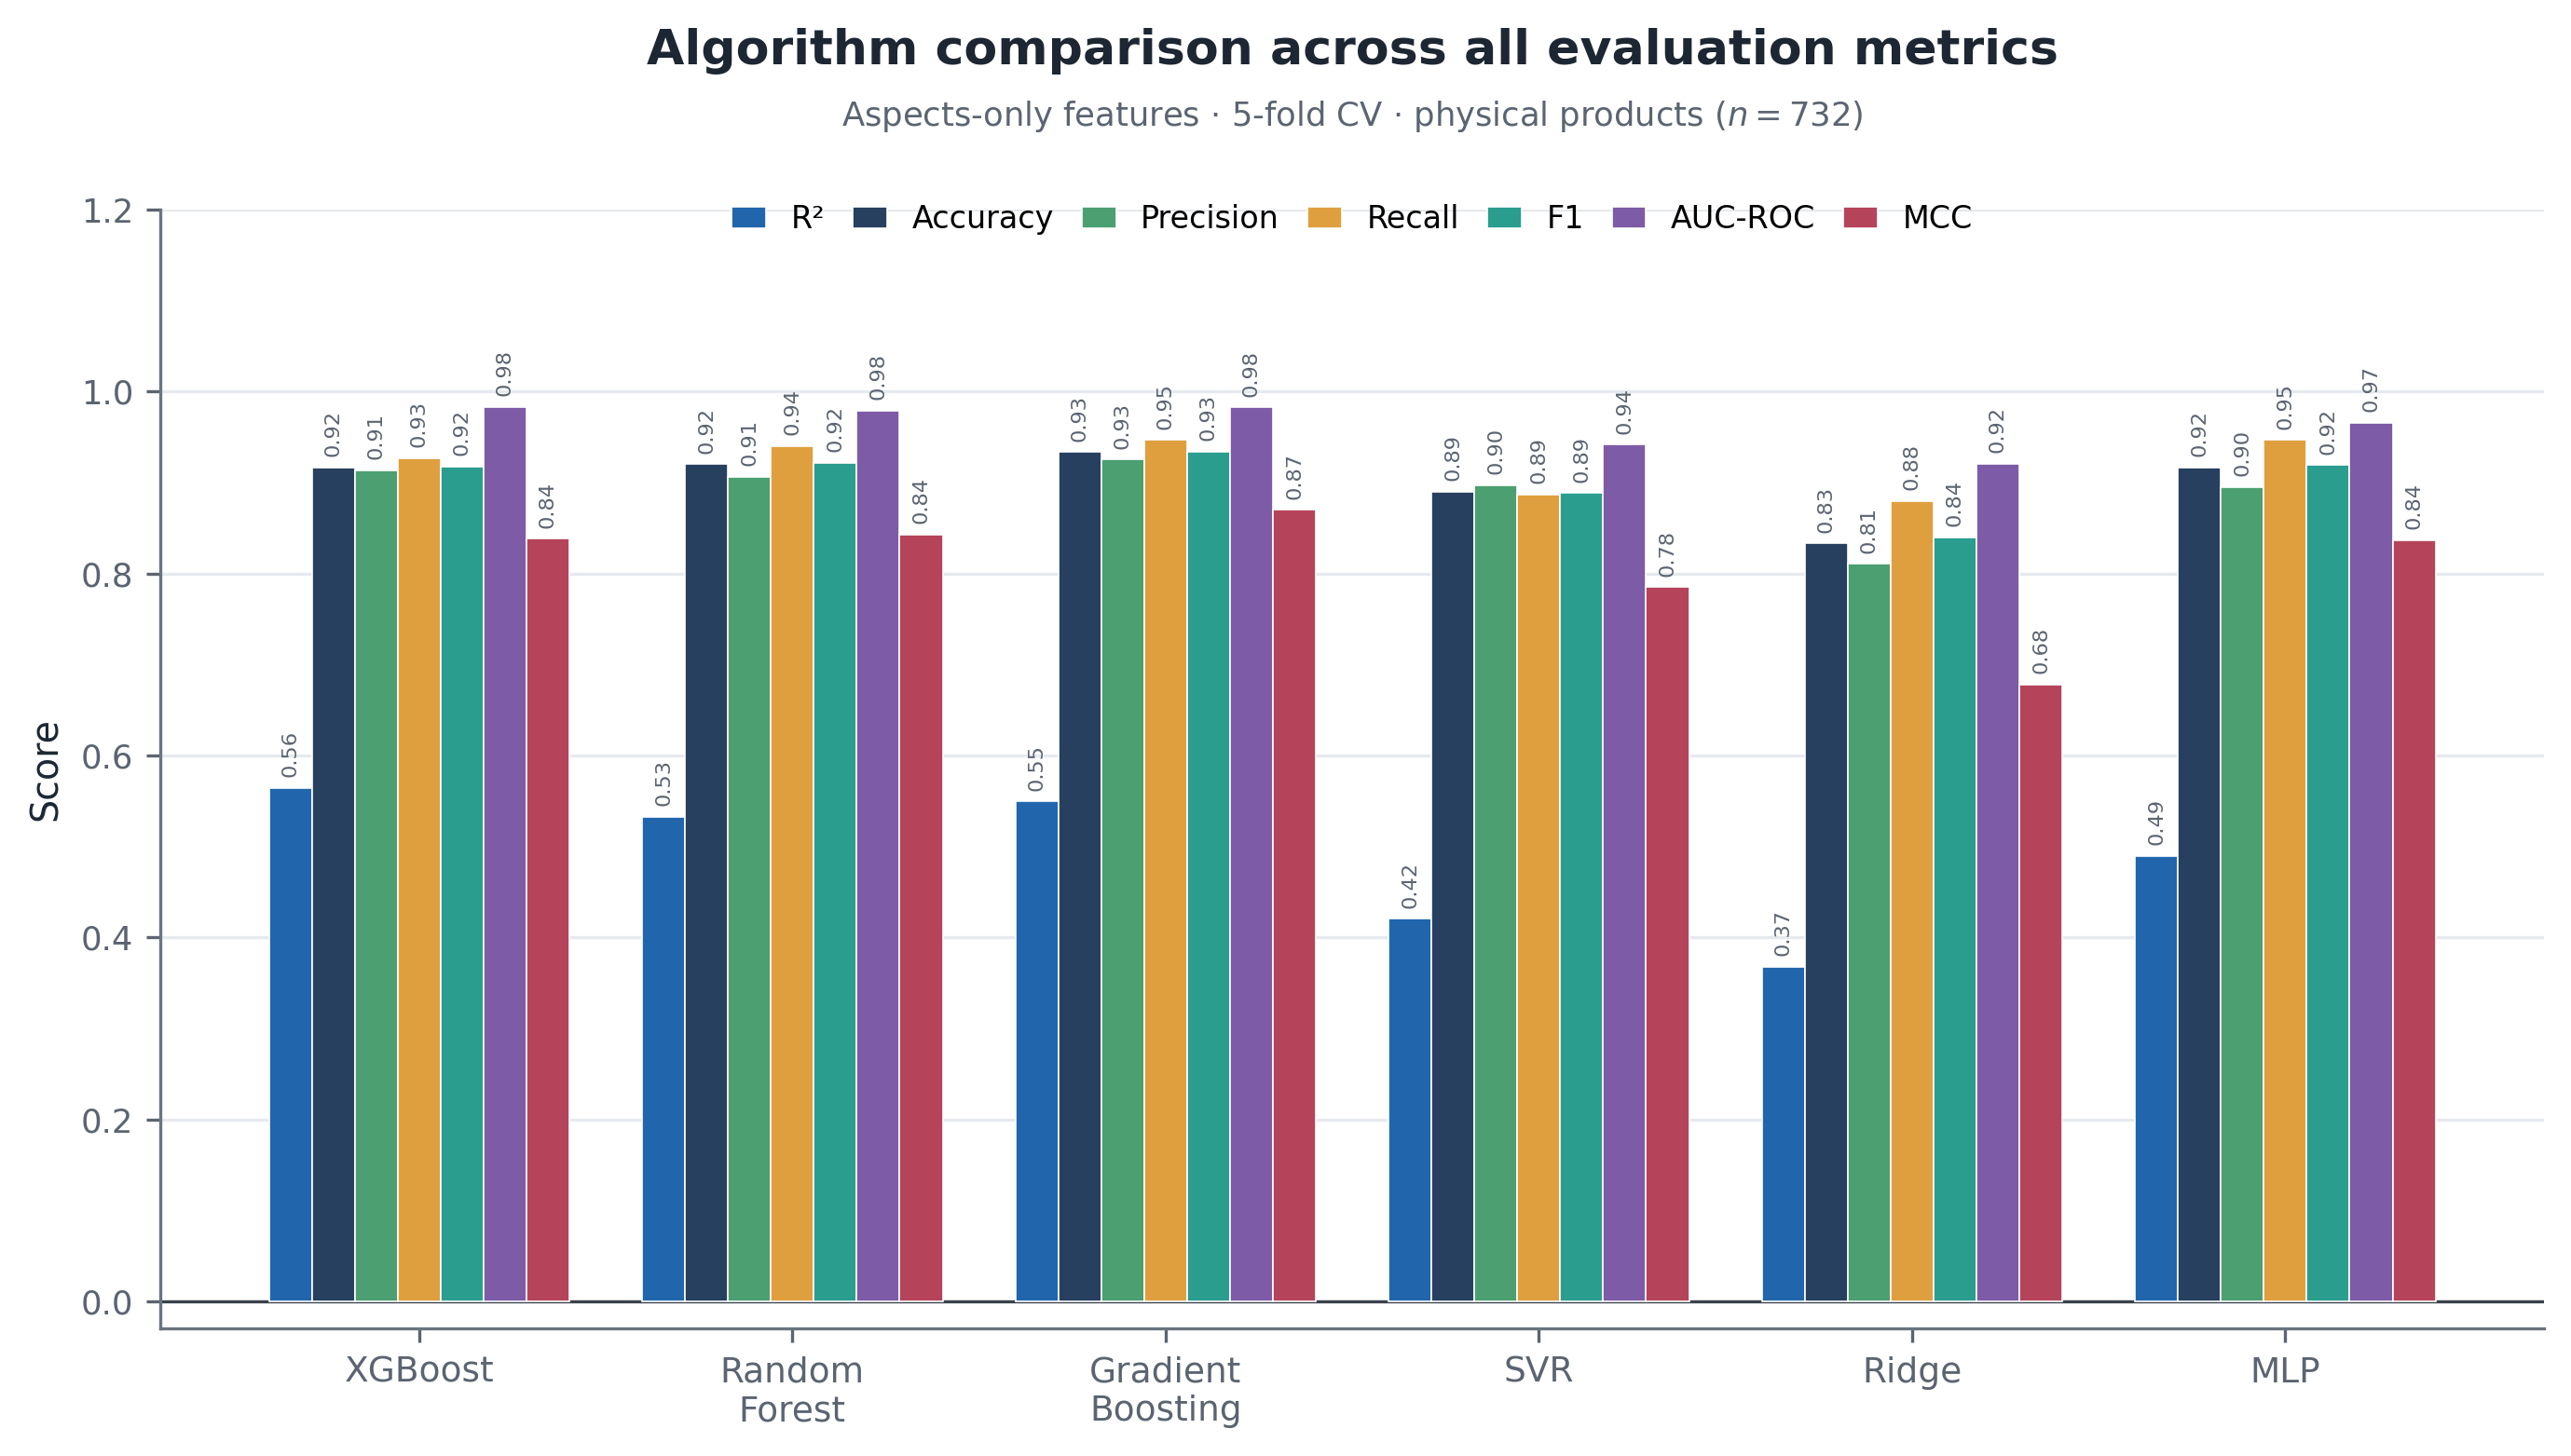
\includegraphics[width=\columnwidth]{fig7_algorithm_metrics.png}
\caption{All evaluation metrics across six algorithms on the aspects-only feature set (5-fold CV, $n=631$). Metrics: $R^2$, Accuracy, Precision, Recall, F1, AUC-ROC, and MCC.}
\label{fig:algometrics}
\end{figure}

\begin{figure}[!t]
\centering
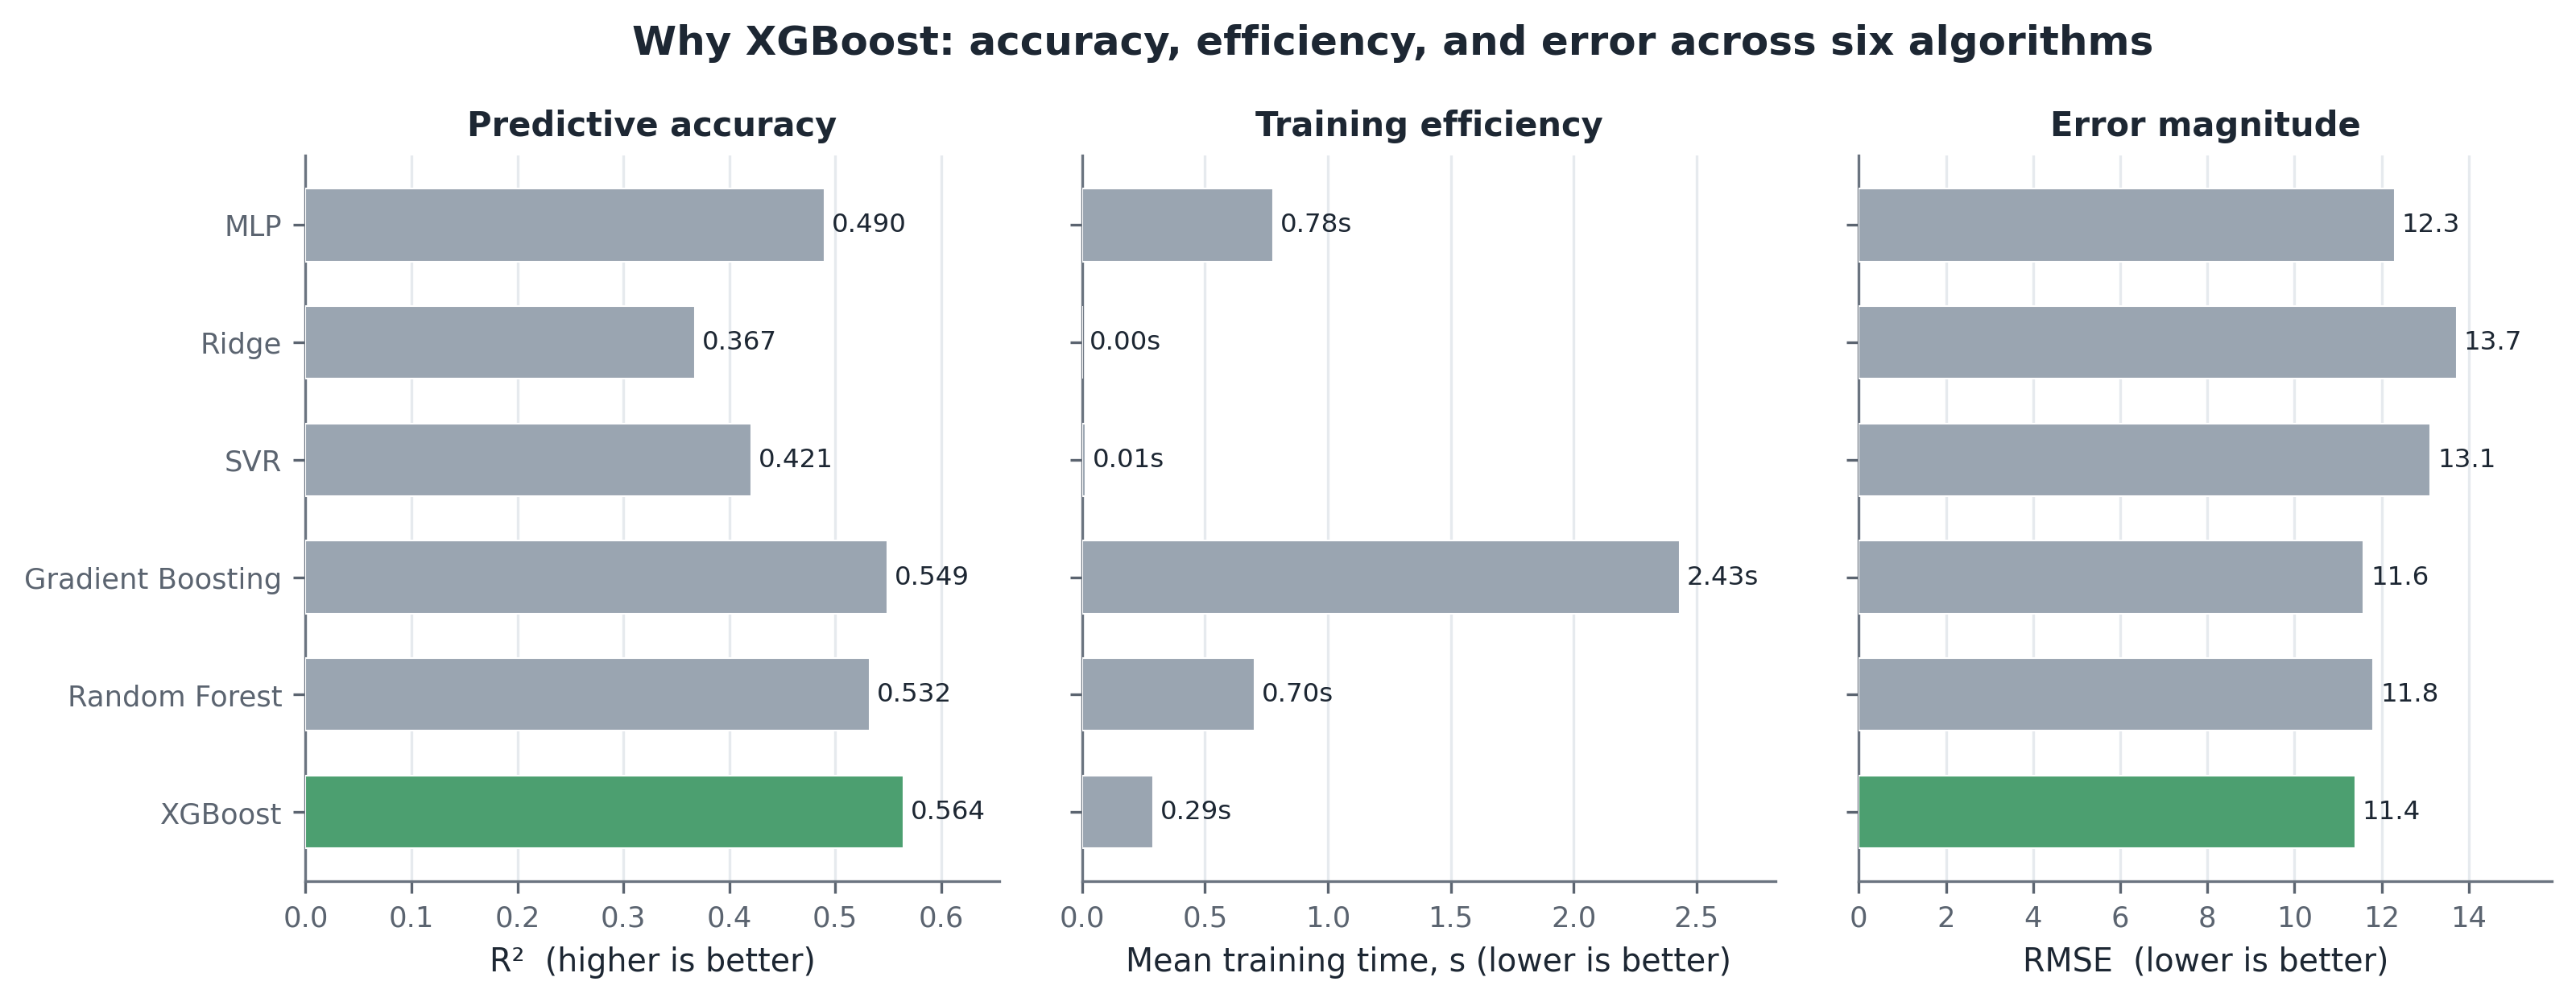
\includegraphics[width=\columnwidth]{fig8_algorithm_tradeoffs.png}
\caption{Three-panel accuracy--efficiency trade-off: predictive accuracy ($R^2$), training time, and error magnitude (RMSE). XGBoost leads on accuracy and error with competitive speed.}
\label{fig:algotradeoffs}
\end{figure}

\begin{figure}[!t]
\centering
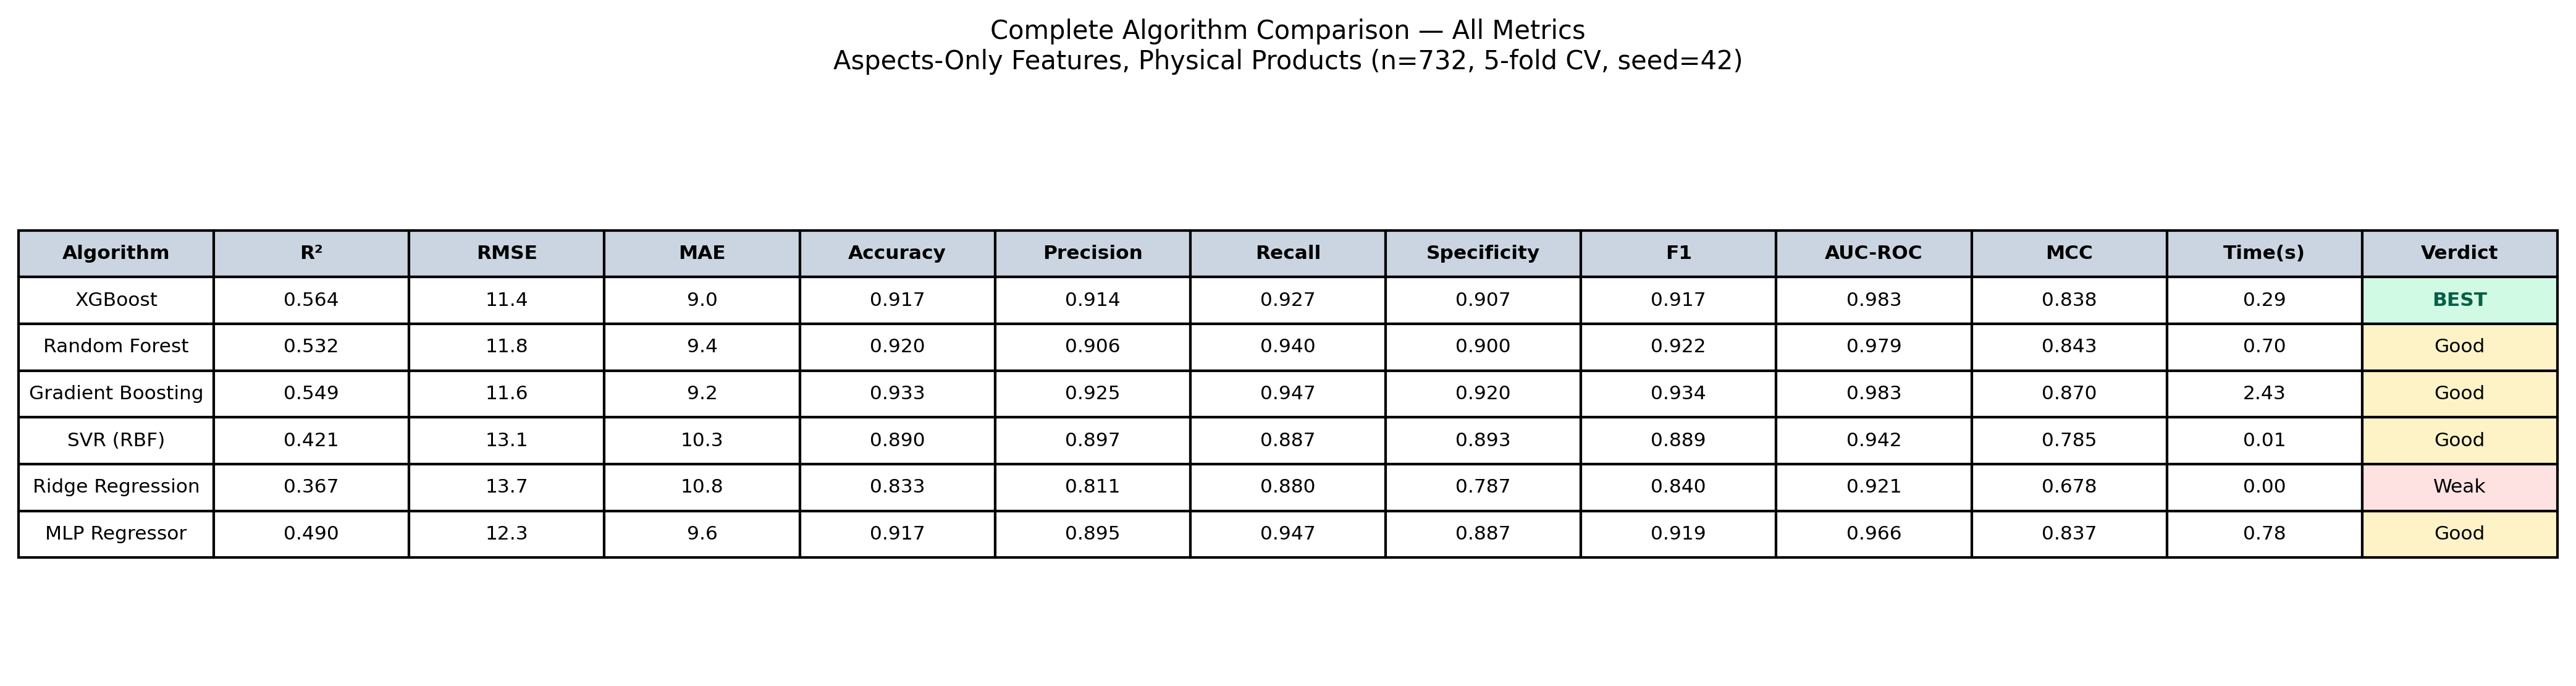
\includegraphics[width=\columnwidth]{fig9_algorithm_table.png}
\caption{Complete numerical comparison across all evaluation metrics. Bold verdict column summarises the overall ranking: XGBoost is the only algorithm rated BEST on both regression accuracy and classification-derived measures while maintaining competitive training time.}
\label{fig:algotable}
\end{figure}

\begin{figure}[!t]
\centering
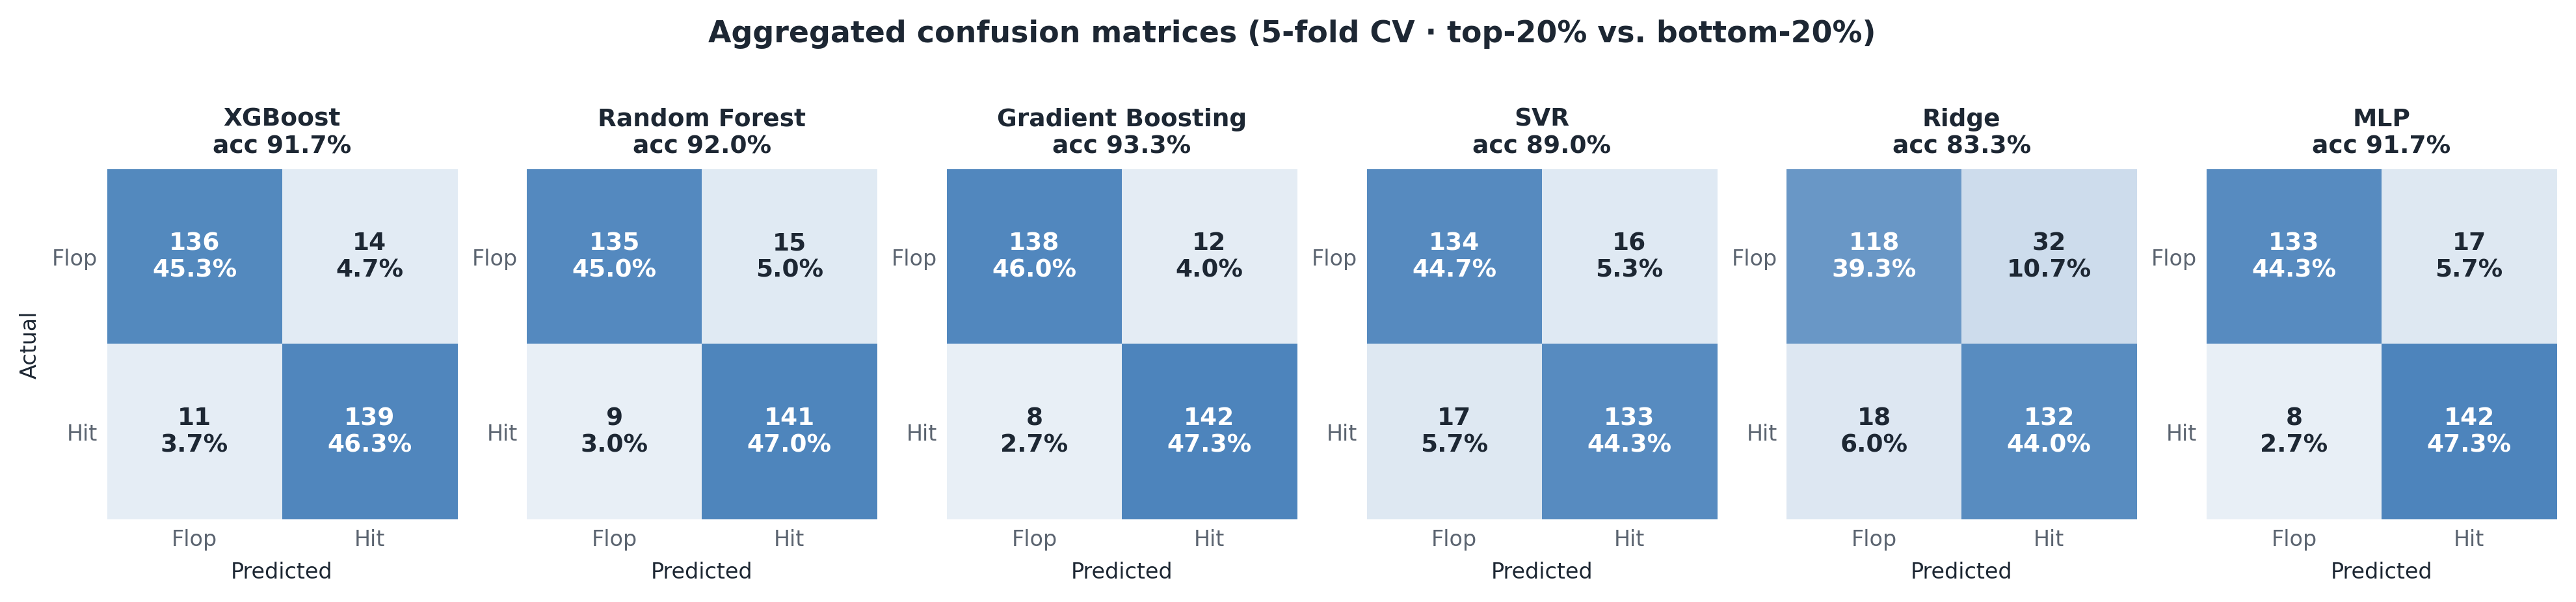
\includegraphics[width=\columnwidth]{fig10_confusion_matrices.png}
\caption{Aggregated confusion matrices (5-fold CV, top-20\% vs.\ bottom-20\% products). Counts and percentages for each quadrant: true negatives (flops correctly identified), false positives, false negatives, and true positives (hits correctly identified).}
\label{fig:confmat}
\end{figure}

\subsection{Bridging: Estimating Aspects from Specifications}
The bridging layer asks an LLM to estimate the aspect profile a product \emph{would} earn after months of real use, given only its specification and a category profile: price quartiles, mean aspect scores, and the top pain points and strengths mined from real reviews. Our first prompt trusted its input, and it failed in a useful way. Marketing copy is optimistic by design, promoting flops and hits with the same enthusiasm, and the predictions collapsed into a narrow optimistic band. The production prompt rests on three skeptic rules. Under \emph{adjective blindness}, only verifiable facts can justify a score, meaning materials, standards, numbers, and warranty terms: ``powerful bass'' is noise, while ``50\,mm drivers'' is evidence. Under the \emph{absence rule}, a spec that offers no concrete evidence for an aspect is treated as a signal in itself, since a competent team states its strengths, so the aspect is scored below the category mean and flagged as ungrounded. Under \emph{anchor discipline}, the category mean is what the median real product achieves, and any score more than two points above it has to cite a spec fact.

\subsection{The Honesty Layer}
Bridged estimates are more reliable for some aspects than others, and the system measures that reliability directly and acts on it rather than hiding it. We compute, per aspect, the correlation between the bridged estimate and the review-derived ground truth across all bridged products (Section~\ref{sec:validation}); this yields an empirical fidelity weight for each aspect. Confidence in a prediction is then a \emph{reliability-weighted} grounded fraction: each aspect contributes to confidence in proportion to how well it actually bridges, so aspects a spec cannot convey (after-sales, $r \approx 0.07$) no longer move confidence, while high-fidelity aspects (utility, durability, ease of use, build quality, reliability, all $r \approx 0.5$) carry it. Each aspect also displays a trust badge from the same measurement: STRONG (utility, ease of use, build quality, durability, reliability), MODERATE (value for money, repairability), or WEAK (design appeal, after-sales). When confidence falls below a warning threshold the interface explains that the estimate leans on category averages; below a lower threshold it suppresses the number entirely and redirects the user to the spec coach. The headline viability is rank-calibrated onto a readable 0--100 scale against a reference distribution of real products, and shown as a range rather than a false-precision decimal.

\begin{figure}[!t]
\centering
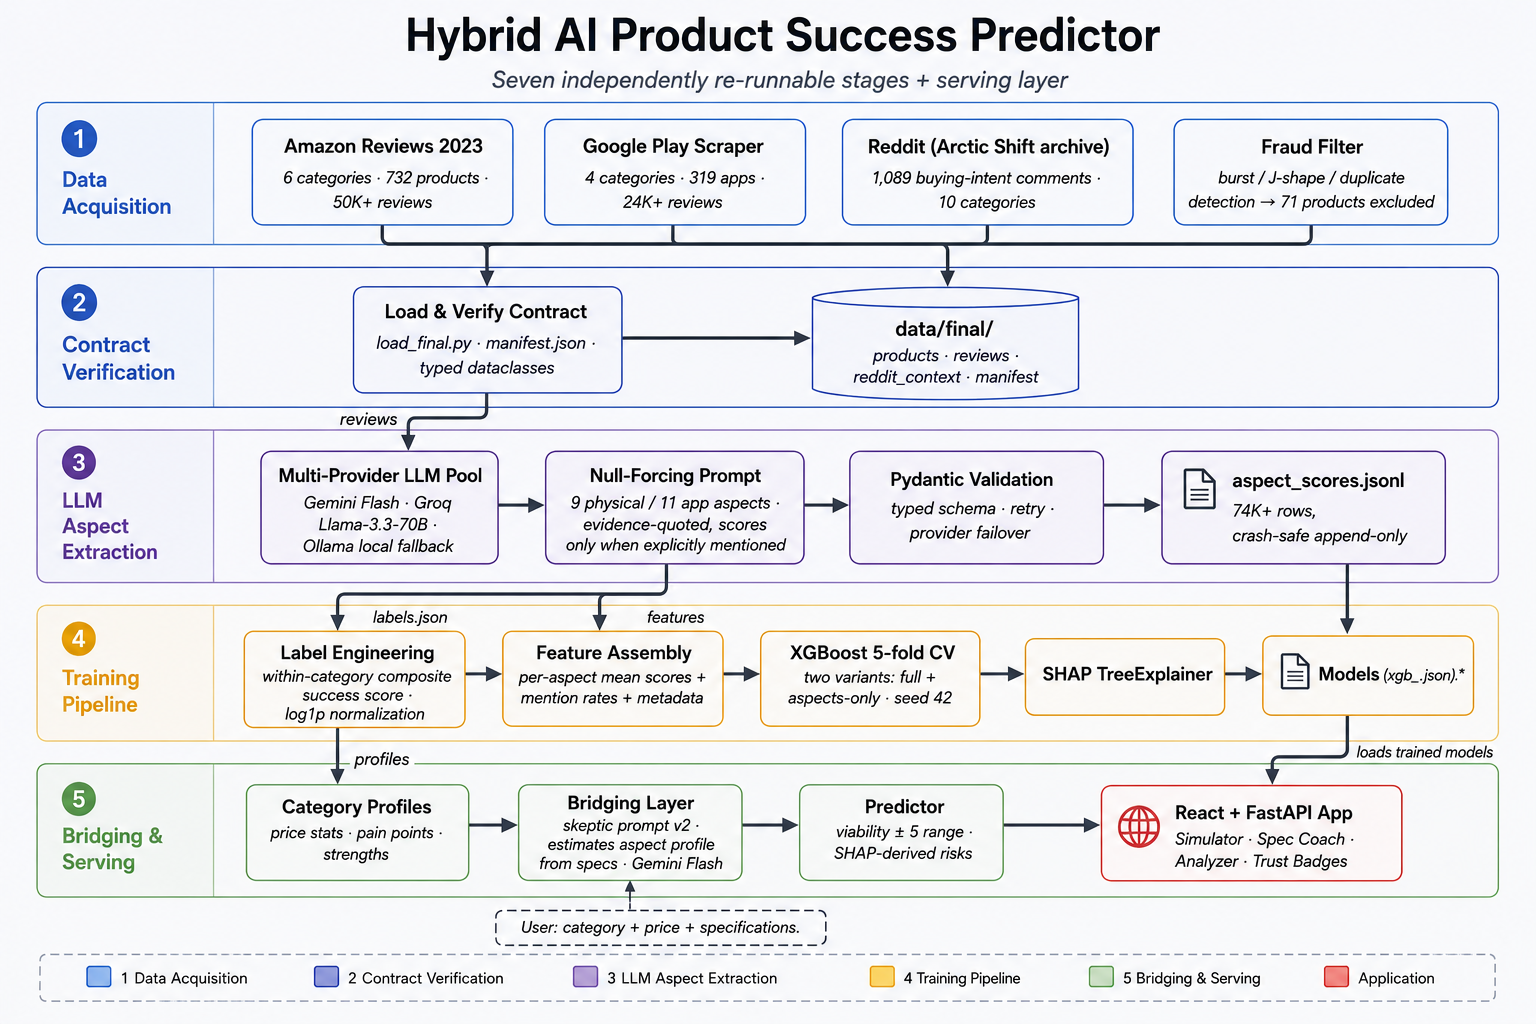
\includegraphics[width=\columnwidth]{fig1_pipeline.png}
\caption{Pipeline overview across five physical categories: extraction, label engineering, feature assembly, training, category profiling, and the bridging/prediction service.}
\label{fig:pipeline}
\end{figure}

\section{Validation}
\label{sec:validation}
The central validation question is a counterfactual: \emph{had our system existed on the day a real product launched, would its specs-only estimate have anticipated that product's eventual market outcome?} We answer it launch-blind and out-of-sample. For each evaluated product, the bridging layer saw only what was knowable at launch: name, brand, price, and the manufacturer's specification copy. Reviews, ratings, and sales signals were withheld. The bridged profile went into the aspects-only model, and its estimate was compared against the product's actual within-category success score, computed from the reviews it later accumulated. Table~\ref{tab:validation} summarizes the three evaluations; the two holdouts are the evidence.

\begin{table}[!t]
\centering
\caption{Reliability summary. The two out-of-sample holdouts are the primary evidence; both scales run 0 (useless) to 1 (perfect). Within-category $\rho$ is the mean over categories and is the stricter measure (Section~\ref{sec:boundary}).}
\label{tab:validation}
\footnotesize
\begin{tabular}{@{}lccc@{}}
\toprule
Evaluation & $\rho$ (pooled) & AUC & within-cat.\ $\rho$ \\
\midrule
Cross-validation ($R^2$) & \multicolumn{3}{c}{$R^2 = 0.603$ aspects-only ($0.566$ pure); $0.893$ full} \\
Out-of-sample holdout ($n{=}118$) & 0.437 & 0.826 & 0.39 \\
Temporal holdout ($n{=}125$) & 0.559 & 0.925 & 0.16 \\
\bottomrule
\end{tabular}
\end{table}

\subsection{Leakage-Controlled Out-of-Sample Holdout}
118 products, spanning all five categories, were bridged with the frozen production pipeline from their specifications. The model was then \emph{retrained from scratch on the other 513 products}, with every holdout product excluded and category priors computed on the training split only, so no test item can influence the model that scores it. Specs-only predictions rank the held-out products against their actual outcomes at Spearman $\rho = 0.437$ ($p = 7.6\times10^{-7}$), with a 10{,}000-sample bootstrap 95\% CI of $[0.275, 0.576]$ that excludes zero, and separate bottom-quintile from top-quintile products at AUC $= 0.826$. Mean predicted viability rises monotonically across the actual success quintiles ($55.4 \to 58.1 \to 58.5 \to 62.8 \to 65.4$; Fig.~\ref{fig:holdout}), a spread of ten points. At $n = 118$ the pooled $\rho$ explains on the order of 19\% of the rank variance; this is a screening signal for a portfolio of candidate designs, not a verdict on any one product.

\begin{figure}[!t]
\centering
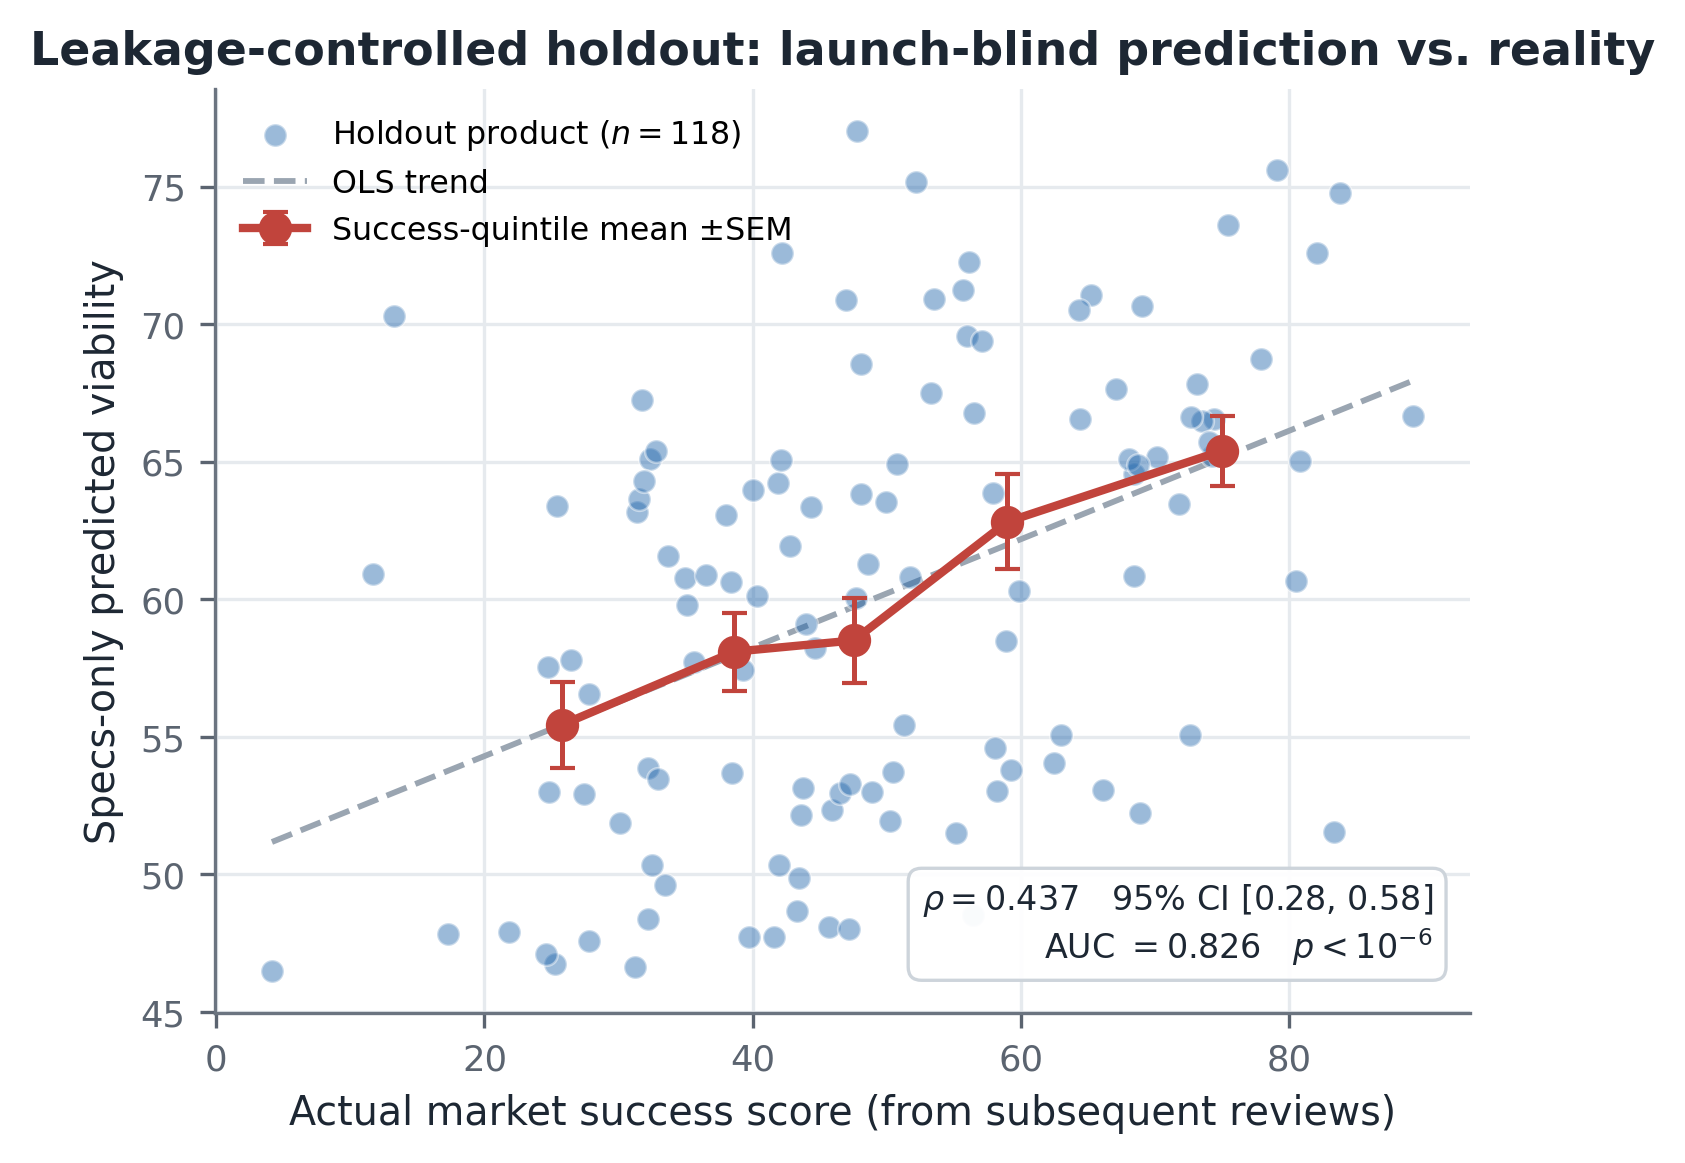
\includegraphics[width=\columnwidth]{fig2_holdout_scatter.png}
\caption{Leakage-controlled holdout ($n=118$): specs-only predicted viability versus actual market success, with monotonic success-quintile means.}
\label{fig:holdout}
\end{figure}

\subsection{Forward-in-Time Temporal Holdout}
A random split can still leak era-specific regularities, so we ran the stricter test a pre-launch tool actually faces: forecasting the future. We trained only on the 505 products launched on or before October~2021 (best iteration selected by 5-fold CV) and predicted the 125 products launched afterward, from specifications alone. The pooled ranking not only holds but tightens: $\rho = 0.559$ ($p = 1.2\times10^{-11}$, CI $[0.429, 0.666]$) and AUC $= 0.925$. That the signal survives a temporal split pre-empts the most common objection to a pre-launch claim.

The pooled numbers, however, benefit partly from \emph{between-category} structure, because the success target is normalized within category. The stricter measure is the mean within-category $\rho$, and here the two holdouts diverge honestly: $0.39$ on the random split falls to $0.16$ forward-in-time. Forecasting the future within a category is genuinely harder than interpolating a random split, which is exactly what a temporal test should expose. We report both and treat the within-category figure as the conservative claim.

\subsection{Baselines and Price Orthogonality}
A launch-blind correlation only matters if it is not just rediscovering price. On the holdout, a within-category price-percentile baseline reaches $\rho = 0.386$ against actual success---a strong baseline, since expensive segments succeed differently. The aspects-only model, which excludes price by construction, reaches $\rho = 0.437$ and is largely orthogonal to price ($r = 0.147$ between prediction and price percentile). The model modestly beats the price baseline while carrying information price position does not, and, unlike a price heuristic, it explains \emph{why} at the level of design levers.

\subsection{Which Aspects Can Be Estimated from Specs}
Per aspect, the bridged estimates correlate with review-derived ground truth at $r = 0.53$ for utility and durability, $0.52$ for ease of use, $0.51$ for build quality, and $0.50$ for reliability; then $0.34$ for value for money and $0.27$ for repairability; and at the low end, design appeal ($r = 0.21$) and after-sales ($r = 0.07$) are essentially unestimable from a specification (Fig.~\ref{fig:validity}; mean $r \approx 0.39$, $n = 118$). That makes sense: service quality is invisible on a spec sheet, and aesthetics are subjective in a way category norms do not capture. These measured correlations are exactly the weights the honesty layer uses, so the interface's trust badges are not asserted---they are the validation numbers themselves.

\begin{figure}[!t]
\centering
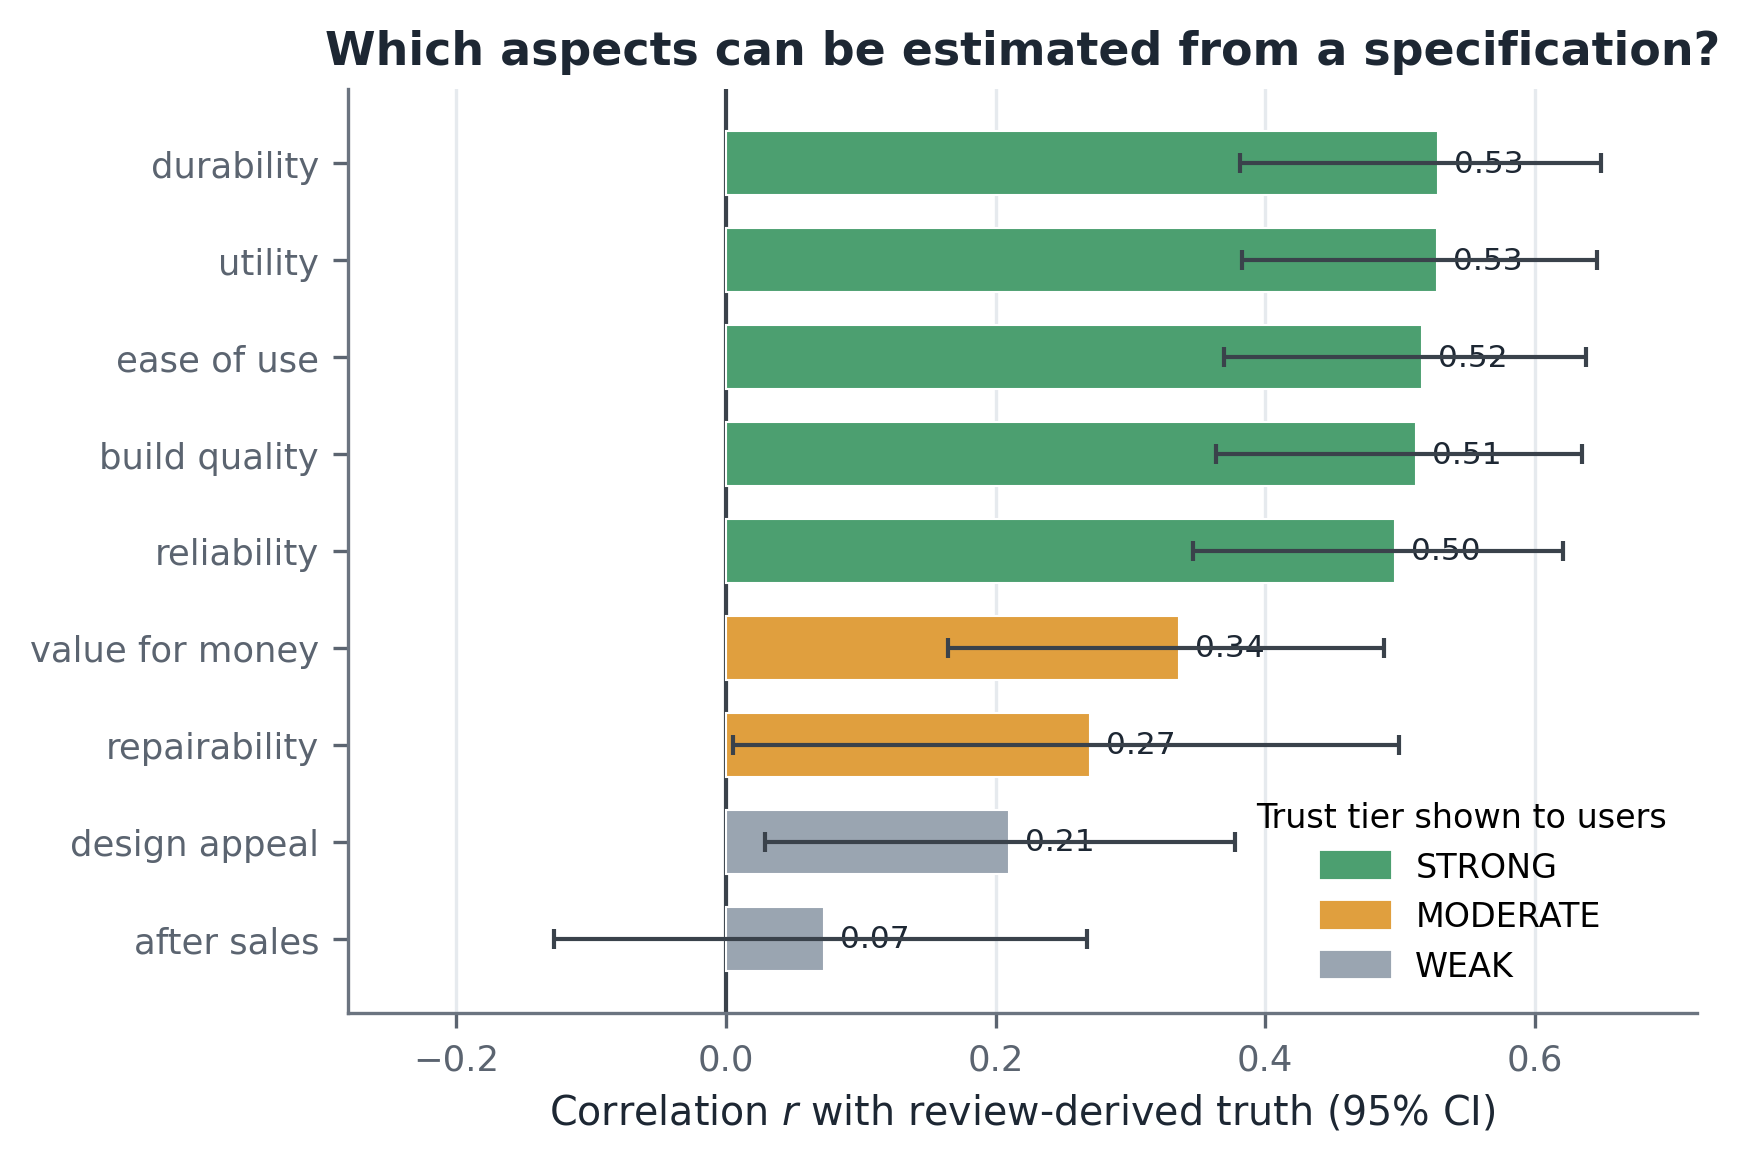
\includegraphics[width=\columnwidth]{fig3_aspect_validity.png}
\caption{Per-aspect validity of bridged estimates ($r$ with 95\% CI, $n=118$), colored by the trust tier shown to users. These correlations double as the confidence weights.}
\label{fig:validity}
\end{figure}

\section{Scope and Boundary Conditions}
\label{sec:boundary}
A system meant to inform real decisions should say where it stops working as clearly as where it works, so we report a diagnosed boundary condition with the same prominence as the positive results. The method's predictive validity tracks \emph{how well a category's specifications encode experiential quality}, and the clearest evidence is the ice-maker category.

Ice makers are, on the surface, the puzzle: they have the \emph{strongest} within-category relationship between real review aspects and success of any category (mean $|r| = 0.32$ against $0.09$--$0.24$ elsewhere) and the best aspect coverage in extraction, yet their bridged predictions are the weakest (holdout $\rho \approx 0.11$; forward-in-time $\rho \approx 0$). The diagnosis is unambiguous and it is not an extraction or label problem: it is the bridging step. The LLM assigns nearly identical aspect scores to every ice maker---bridged-score standard deviation across products of $0.08$ for reliability, $0.13$ for build quality and durability---because ice-maker specifications are capacity-and-speed numbers (``26\,lb/day, 9 cubes in 6 minutes'') that convey nothing about reliability, durability, or build. With no basis to differentiate, the model defaults every product to the category prior, and flat inputs carry no ranking information. Ice-maker bridging fidelity is therefore $r \approx 0.04$, against $\approx 0.39$ pooled and $0.45$--$0.56$ for the same aspects in personal-electronics categories.

The lesson generalizes. Where a category's specifications describe experiential attributes---sound, comfort, battery life for headphones, speakers, and smartwatches---bridging fidelity is high and forward prediction works. Where they describe only physical capacity, bridging cannot differentiate products and the method is bounded, regardless of how much signal the underlying reviews contain. A related effect appears in the temporal holdout: power banks rank well on a random split ($\rho = 0.43$) but not forward-in-time ($\rho \approx 0$), consistent with genuine technological drift (newer gallium-nitride and USB-C designs) that a model trained on older products has not seen. We therefore scope the method to spec-expressive, technologically stable categories, and the interface's abstention machinery is the runtime expression of the same boundary.

\section{System}
\label{sec:system}
The pipeline runs as independently re-runnable stages (Fig.~\ref{fig:pipeline}). Each stage writes its output to disk and skips expensive work unless forced to redo it. The extraction stage is crash-safe and resumable, which mattered in practice, because the full batch runs for days of rate-limited API calls across a rotating provider pool. Feature manifests are serialized to disk, and the prediction code builds its input vectors by iterating over them, so the serving path can never quietly drift out of alignment with training. A single end-to-end smoke test regenerates synthetic data and runs every stage in a sandbox, and it gates every code change.

The user-facing application (Fig.~\ref{fig:ui}a) is a React front end on a FastAPI backend, deployed under Docker. A founder describes a product by category, price, and specification, and gets the full analysis back: a rank-calibrated viability range, a percentile position against real products, per-aspect estimates plotted against category averages, SHAP-derived \cite{lundberg2017shap} top risks and strengths stated in terms of design levers the founder actually controls, and a market-gap report that quotes verbatim customer complaints for the category pain points the design does not convincingly address. Every aspect estimate carries its trust badge and grounding flag, and confidence is reliability-weighted, so a specification that grounds only low-fidelity aspects is reported at low confidence and, below threshold, replaced by an explanation rather than a number. The model also conditions on company and product maturity, so a first product from an unknown brand is judged differently from a line extension by an established one.

The spec coach (Fig.~\ref{fig:ui}b) closes the loop for users who are not practiced spec writers. One LLM call rates the draft's coverage of each aspect as covered, vague, or missing, asks at most five questions ordered by how much each answer would sharpen the prediction, and rewrites the spec while keeping every stated fact and inserting explicit placeholders for the decisions still to be made. The coach is forbidden, by construction, from inventing any material, number, or feature the user did not state.

\begin{figure}[!t]
\centering
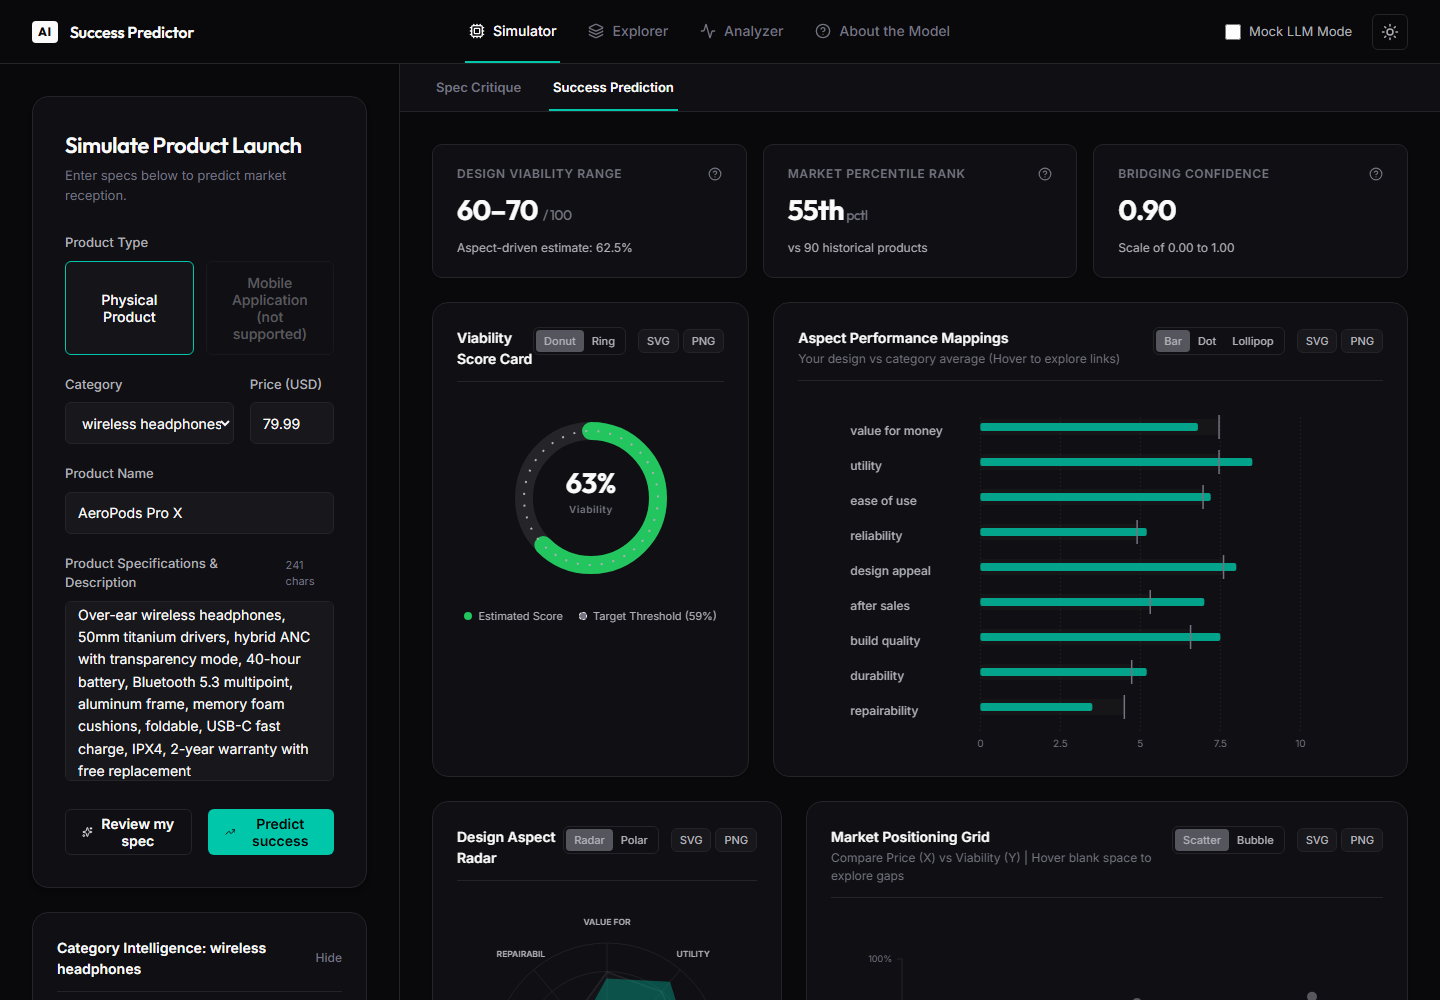
\includegraphics[width=\columnwidth]{fig6a_prediction.png}\\[2pt]
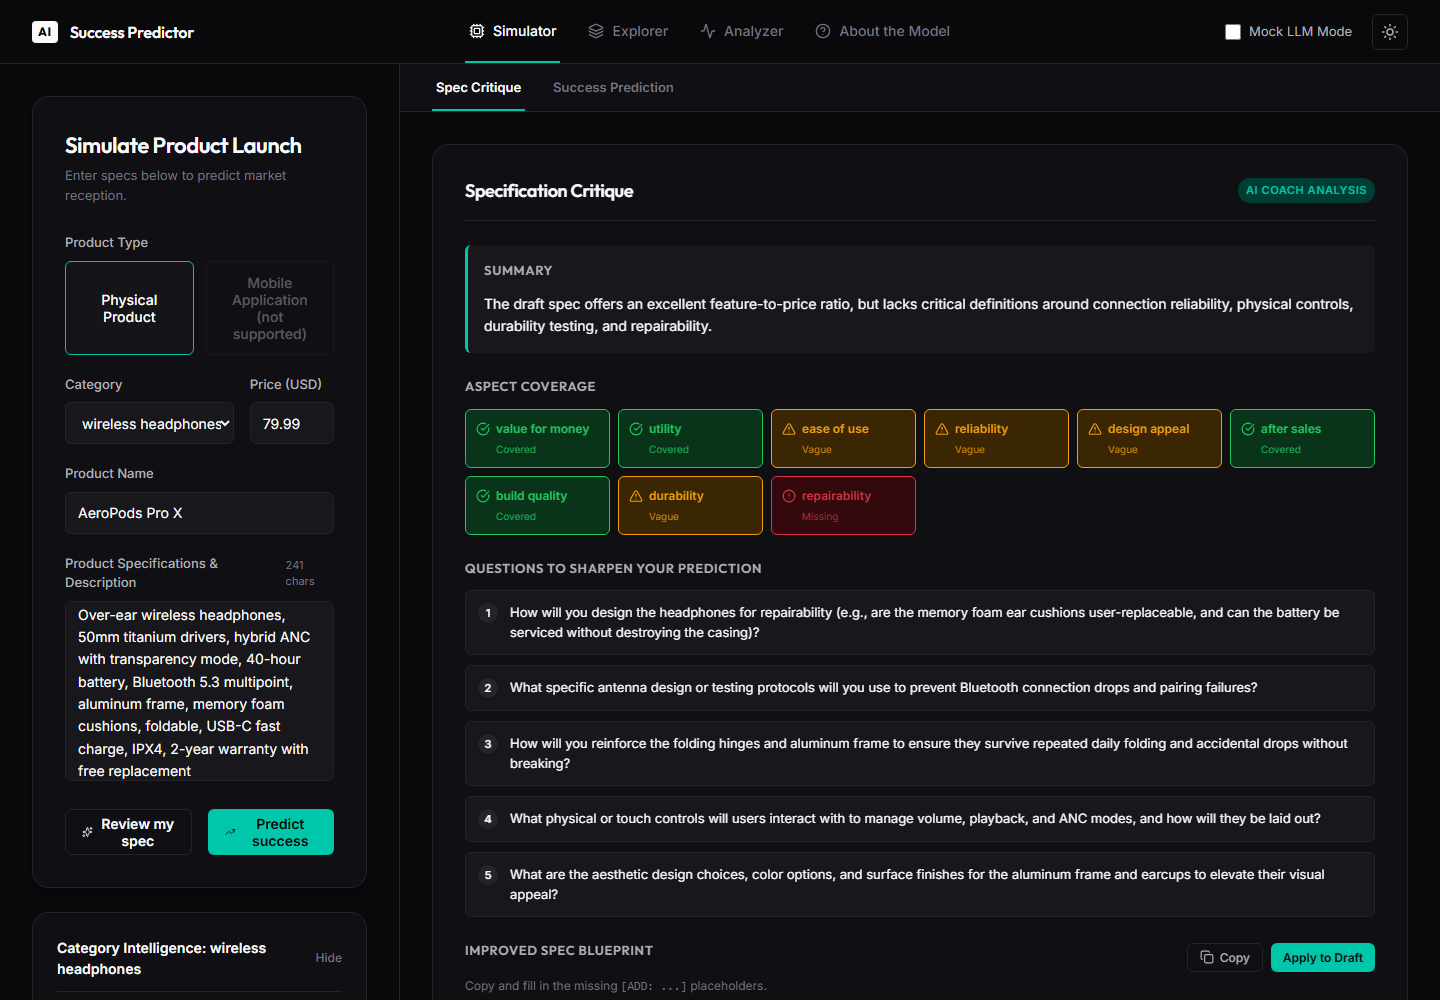
\includegraphics[width=0.49\columnwidth]{fig6b_spec_coach.png}\hfill
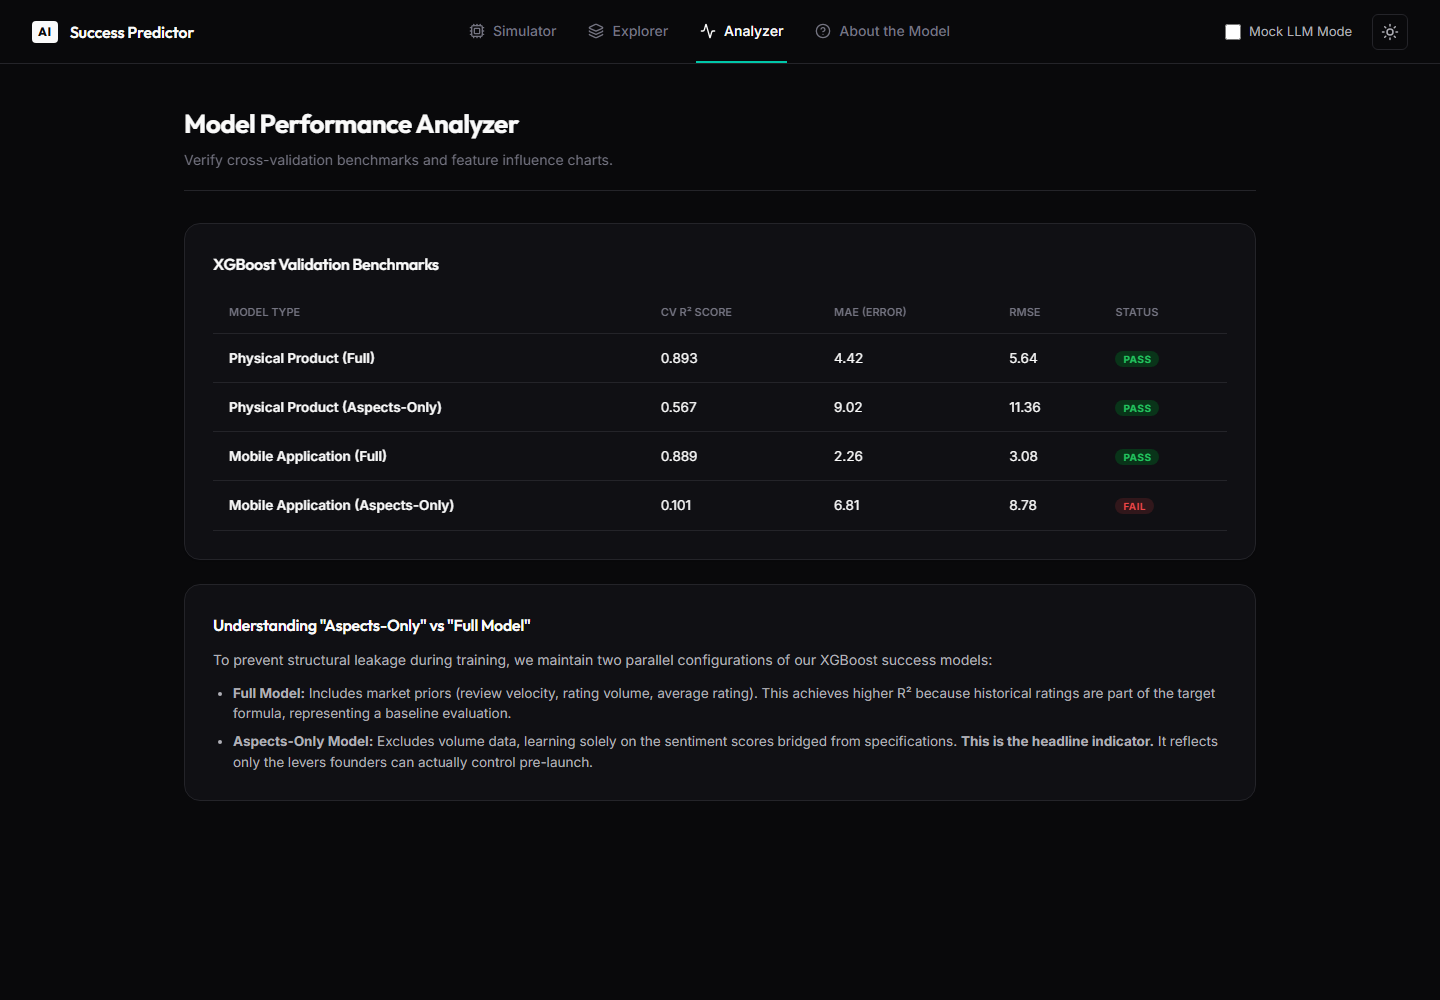
\includegraphics[width=0.49\columnwidth]{fig6c_analyzer.png}
\caption{The application. (a)~Prediction dashboard with viability range, percentile rank, and aspect-vs-category chart. (b)~Spec coach. (c)~Analyzer view showing the honest benchmark table.}
\label{fig:ui}
\end{figure}

\section{Limitations}
\label{sec:limitations}
\textbf{Survivorship bias is the most important limitation, and it bounds every claim in this paper.} The corpus requires at least five reviews per product, so products that launched and drew no attention, arguably the truest flops, are simply absent. Every result here is about ranking among products that reached the market's attention. Whether the system could flag a product destined to gain no traction at all is untested, and with this data it is untestable.

The second limit is the target itself: our success score is a review-derived popularity composite, not units sold, which are not publicly available. A real sales signal (for example, sales rank) is the highest-leverage improvement available. The third is statistical power and scope: the holdouts have $n = 118$ and $125$, the validated claims cover five physical categories, and within-category forward skill is modest ($\rho \approx 0.16$) and concentrated in spec-expressive categories (Section~\ref{sec:boundary}). The fourth concerns the inputs. Our ``specifications'' are launch-day specification and marketing copy, the closest launch-knowable proxy we can recover after the fact, optimistic in ways the skeptic prompt reduces without removing. The fifth is reproducibility: the pipeline depends on hosted LLMs, and while prompts and seeds are frozen, provider models change over time, so exact reproduction needs the archived extraction outputs we publish with the code. Last, review text can be gamed; the fraud filter removed 9 suspect products, but a sophisticated manipulation \cite{mayzlin2014promotional} would slip through it. Incorporating community-derived buying priorities as additional bridging context is a promising but unconfirmed direction we leave to future work.

\section{Conclusion}
We asked whether a product's market fate can be read, at least in part, from its specification alone, before any consumer has touched it. Within carefully stated bounds, the answer is yes. An LLM that extracts aspect sentiment from more than 43{,}000 reviews, a gradient-boosted model that learns which aspect profiles succeed, and a skeptic-prompted bridging layer that estimates those profiles from specs together produce a launch-blind signal of $\rho = 0.437$ on a leakage-controlled holdout and $\rho = 0.559$ forward-in-time, against real market outcomes. It is largely orthogonal to price, and predicted viability rises monotonically across success tiers from flops to category leaders.

The most durable contribution, we think, is not that point estimate but the map around it: which aspects a specification can predict (utility, ease of use, build quality, durability, reliability), which it cannot (after-sales service, aesthetics), and which categories the method works in at all---spec-expressive personal electronics---as against where it is bounded, such as commodity appliances whose specs encode capacity but not experience. For the small businesses that motivated this work, a map like that is the difference between an oracle they should not trust and an instrument they can: a pre-production screen that shifts the odds toward products their users find worth paying for. A tool that knows its own limits and shows them, through reliability-weighted confidence, trust badges, and abstention, is the only honest form such a tool can take at the current state of the art.

\bibliographystyle{IEEEtran}
\bibliography{refs}

\end{document}
